\begin{frame}
  \frametitle{Problem Setup}
  \begin{definition}[Minimum finding]
    Let $T[0..N-1]$ be an unsorted table of $N$ items from an ordered set.

    \vspace{0.3em}
    \textbf{Access:} query oracle $\ket{x}\ket{0}\mapsto\ket{x}\ket{T[x]}$.

    \vspace{0.3em}
    \textbf{Goal:} find $y^*$ such that $T[y^*] = \min_x T[x]$.
  \end{definition}

  \vspace{0.5cm}
  {\small Assume values are distinct for simplicity; the analysis extends to ties.}
\end{frame}

\begin{frame}
  \frametitle{The Threshold Oracle}
  Given a current ``best-so-far'' index $y$, define
  \[
    f_y(x) =
    \begin{cases}
      1, & T[x] < T[y] \\
      0, & T[x] \ge T[y]
    \end{cases}
  \]

  \vspace{0.3cm}
  \begin{itemize}[<+->]
    \item $f_y$ marks exactly the items \textbf{strictly better} than $y$
    \item Implemented by one call to $T$ plus a comparator: $O_g(\log N)$ extra gates
    \item Let $t$ = number of marked items. Then $t$ is the current rank of $y$ minus one
  \end{itemize}

  \vspace{0.4cm}
  \only<4->{\textbf{Feed $f_y$ into $\textsc{ExpSearch}$, keep the winner, repeat.}}
\end{frame}

\begin{frame}
  \frametitle{Algorithmic Idea}
  \begin{itemize}[<+->]
    \item Initialize $y$ at random
    \item Run $\textsc{ExpSearch}(f_y)$ to get some $y'$ with $T[y'] < T[y]$
    \item Update $y \leftarrow y'$
    \item The threshold strictly decreases at each successful round
    \item Repeat until no item is better than $y$; return $y$
  \end{itemize}

  \vspace{0.5cm}
  \only<6->{The number of marked items $t$ shrinks over time,\\
  so each round becomes ``easier but with fewer targets.''}
\end{frame}

\begin{frame}
  \frametitle{Visualizing the Threshold Descent}
  \begin{center}
    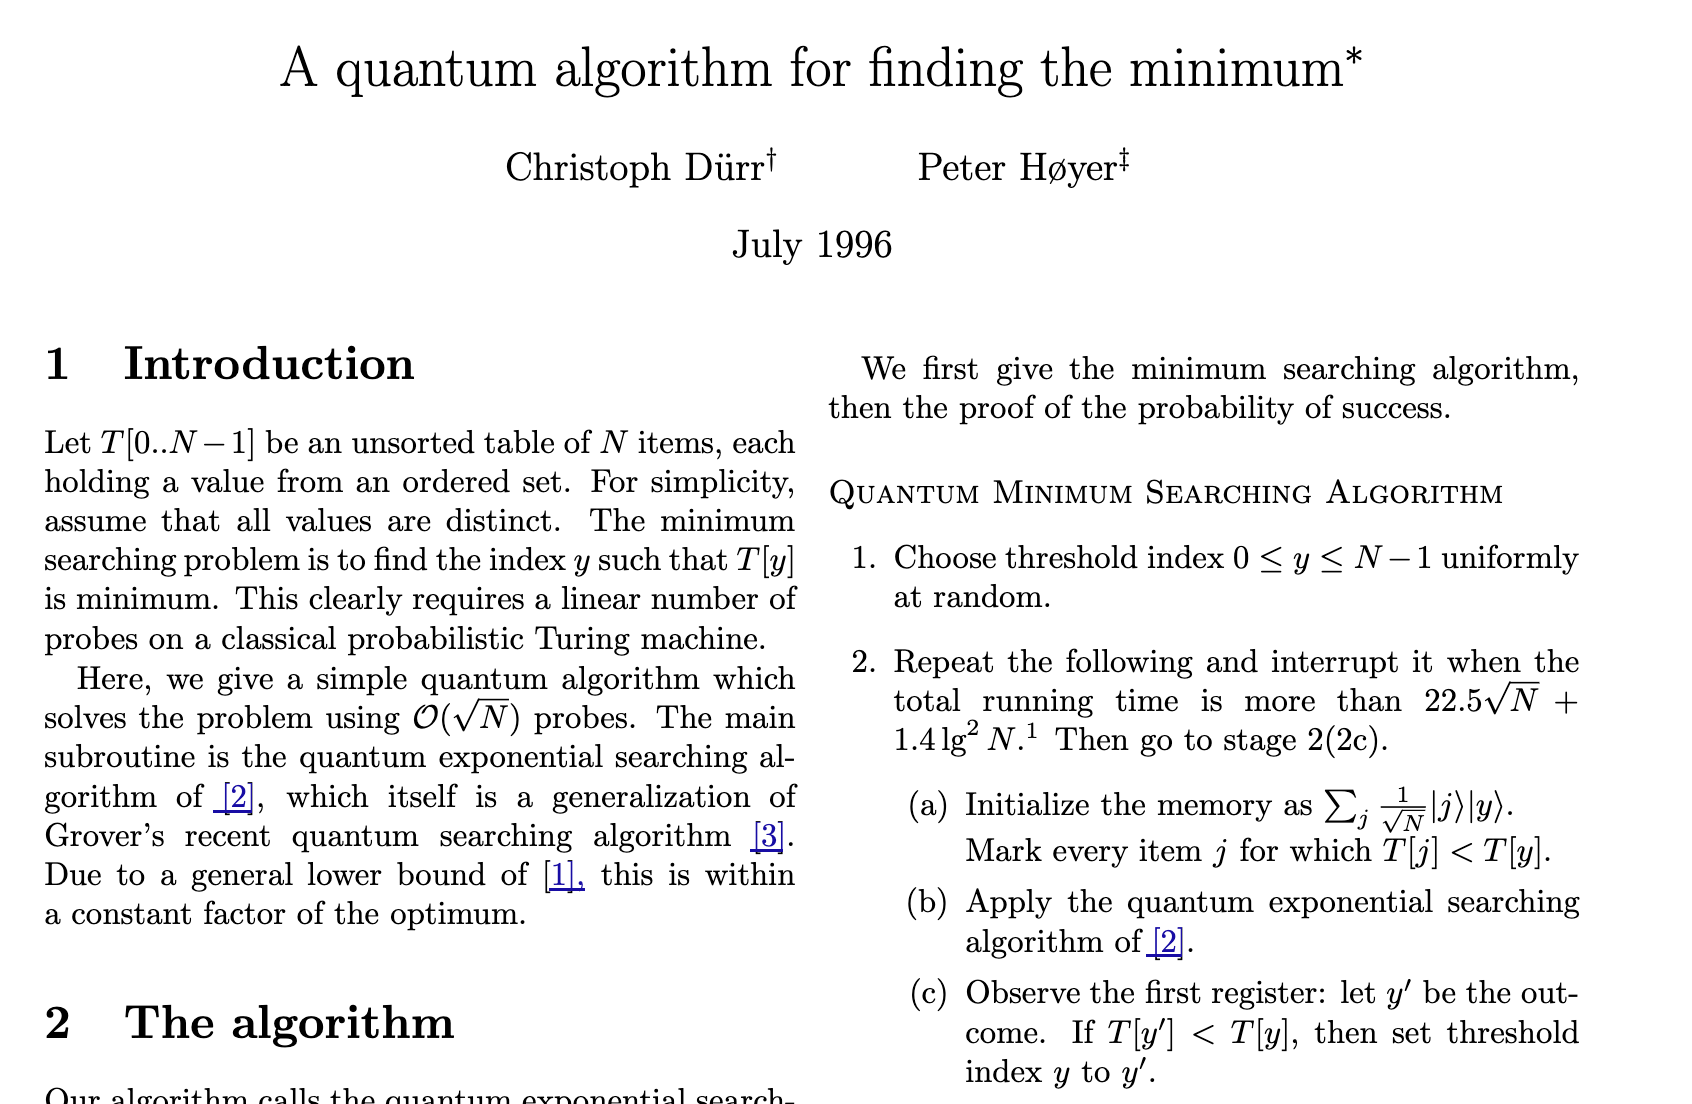
\includegraphics[width=0.95\textwidth,height=0.65\textheight,keepaspectratio]{imgs/algo1_abstract.png}
  \end{center}

  \vspace{0.2cm}
  {\small The threshold $y$ jumps down to a random marked item at each step, until the set of marked items is empty.}
\end{frame}

\begin{frame}
  \frametitle{The D\"urr--H\o yer Algorithm}
  {\small Output: index $y$ with $T[y]$ minimal, w.h.p.}

  \vspace{0.3em}
  \begin{enumerate}
    \item Pick $y \in \{0,\dots,N-1\}$ uniformly at random
    \item Repeat until total time exceeds
      \[
        22.5\sqrt{N} + 1.4 \lg^2 N
      \]
    \begin{enumerate}
      \item Prepare $\tfrac{1}{\sqrt{N}}\sum_j \ket{j}\ket{y}$; mark $j$ iff $T[j] < T[y]$
      \item $y' \leftarrow \textsc{ExpSearch}(f_y)$
      \item If $T[y'] < T[y]$, set $y \leftarrow y'$
    \end{enumerate}
    \item Return $y$
  \end{enumerate}

  \vspace{0.4em}
  {\small Time budget: one Grover iteration = one time step; preparing stage 2(a) costs $\lg N$.}
\end{frame}

\section{Analysis}

\begin{frame}
  \frametitle{Analysis Roadmap}
  \begin{itemize}[<+->]
    \item Pretend we never time out (``infinite algorithm'')
    \item Show: item of rank $r$ becomes threshold with probability $1/r$
    \item Sum contributions $\Rightarrow$ expected runtime is $O(\sqrt{N})$
    \item Markov $\Rightarrow$ running $2\times$ longer gives success probability $\ge 1/2$
  \end{itemize}

  \vspace{0.4cm}
  \only<5->{\textbf{Everything follows from one clean lemma on rank probabilities.}}
\end{frame}

\begin{frame}
  \frametitle{Lemma 1: Rank Probability}
  \begin{lemma}[D\"urr--H\o yer]
    Let $p(t, r)$ be the probability that the item of rank $r$ ever becomes the threshold, when the infinite algorithm starts with $t$ marked items. Then
    \[
      p(t, r) =
      \begin{cases}
        1/r, & r \le t \\
        0, & r > t
      \end{cases}
    \]
  \end{lemma}

  \vspace{0.4cm}
  \begin{itemize}
    \item Rank $r$: the $r$-th smallest element
    \item Remarkably, the probability does not depend on $t$
    \item Rank 1 (the true minimum) is hit with probability 1
  \end{itemize}
\end{frame}

\begin{frame}
  \frametitle{Proof of Lemma 1}
  Induction on $t$ for fixed $r$.

  \vspace{0.3cm}
  \textbf{Base:} $p(r, r) = 1/r$ because AA returns a uniform marked index.

  \vspace{0.3cm}
  \textbf{Step:} assume $p(k,r) = 1/r$ for all $k \in [r, t]$. With $t+1$ marked items:
  {\small
  \[
    p(t+1, r) = \underbrace{\tfrac{1}{t+1}}_{\text{hit $r$ now}}
    + \sum_{k=r+1}^{t+1} \tfrac{1}{t+1}\, p(k-1, r)
  \]
  \[
    = \tfrac{1}{t+1} + \tfrac{t+1-r}{t+1}\cdot\tfrac{1}{r}
    = \tfrac{1}{r}.
  \]
  }

  \vspace{0.3cm}
  {\small Cases where the chosen item has rank $<r$ contribute $0$ (rank $r$ stops being marked).}
\end{frame}

\begin{frame}
  \frametitle{Lemma 2: Expected Runtime}
  \begin{lemma}
    The expected total time used by the infinite algorithm before $y$ holds the index of the minimum is at most
    \[
      m_0 = \tfrac{45}{4}\sqrt{N} + \tfrac{7}{10}\lg^2 N.
    \]
  \end{lemma}

  \vspace{0.3cm}
  Two pieces:
  \begin{itemize}
    \item \textbf{AA calls:} $\sum_r p(N,r)\cdot \tfrac{9}{2}\sqrt{N/(r-1)}$
    \item \textbf{Oracle prep:} $\sum_r p(N,r)\cdot \lg N$
  \end{itemize}
\end{frame}

\begin{frame}
  \frametitle{Proof of Lemma 2 (AA part)}
  {\small
  \[
    \sum_{r=2}^{N} p(N,r)\,\tfrac{9}{2}\sqrt{\tfrac{N}{r-1}}
    = \tfrac{9}{2}\sqrt{N}\sum_{r=1}^{N-1}\tfrac{1}{r+1}\cdot\tfrac{1}{\sqrt{r}}
  \]
  \[
    \le \tfrac{9}{2}\sqrt{N}\left(\tfrac{1}{2} + \sum_{r=2}^{N-1} r^{-3/2}\right)
    \le \tfrac{9}{2}\sqrt{N}\left(\tfrac{1}{2} + \int_1^{N-1} r^{-3/2}\,dr\right)
  \]
  \[
    = \tfrac{9}{2}\sqrt{N}\left(\tfrac{1}{2} + \left[-2r^{-1/2}\right]_1^{N-1}\right)
    \le \tfrac{45}{4}\sqrt{N}.
  \]
  }

  \vspace{0.5cm}
  {\small For oracle prep: $\sum_r p(N,r)\lg N = (H_N - 1)\lg N \le \ln N \lg N \le \tfrac{7}{10}\lg^2 N$.}
\end{frame}

\begin{frame}
  \frametitle{Theorem 1: Success Probability}
  \begin{theorem}[D\"urr--H\o yer \cite{durr1996minimum}]
    With time-out $2 m_0 = 22.5\sqrt{N} + 1.4\lg^2 N$, the algorithm outputs the index of the minimum with probability at least $1/2$.

    \vspace{0.3em}
    Its running time is $O(\sqrt{N})$.
  \end{theorem}

  \vspace{0.5cm}
  \begin{itemize}[<+->]
    \item Markov: $\Pr[\text{runtime} > 2 m_0] \le 1/2$
    \item So with probability $\ge 1/2$ the infinite algorithm has already reached the minimum
    \item Boosting: run $c$ copies, take the best $\Rightarrow$ error $\le 1/2^c$
  \end{itemize}
\end{frame}

\begin{frame}
  \frametitle{Why This Is Tight}
  \begin{itemize}[<+->]
    \item Min finding $\ge$ unstructured search (a marked item is just the minimum of a $0$/$1$ table)
    \item By BBBV\,\cite{bennett1997strengths}, $\Omega(\sqrt{N})$ queries are required
    \item So D\"urr--H\o yer is \textbf{asymptotically optimal}
  \end{itemize}

  \vspace{0.5cm}
  \only<4->{\textbf{Grover is the lower bound; D\"urr--H\o yer matches it for a strictly harder task.}}
\end{frame}

\begin{frame}
  \frametitle{What About the Maximum?}
  \begin{itemize}[<+->]
    \item Flip the comparator: $f_y(x) = 1$ iff $T[x] > T[y]$
    \item Same algorithm, same analysis, same $O(\sqrt{N})$
    \item Ahuja--Kapoor gave an explicit write-up\,\cite{ahuja1999maximum}
  \end{itemize}

  \vspace{0.4cm}
  \only<4->{So we have \textbf{min, max, arg-min, arg-max} all in $O(\sqrt{N})$.}
\end{frame}

\begin{frame}
  \frametitle{Quick check}
  \begin{center}
    
\includegraphics[width=0.8\textwidth,height=0.6\textheight,keepaspectratio]{imgs/survey_1.png}
  \end{center}

  Any issues with Lemma~1 or the runtime bound before we go to $k$-minima?
\end{frame}
